%!TEX root=../oi-magistr-spolecne.tex
\section[PAL - Stromy]{Vyhledávací stromy: B, B+, R-B, 2-3-4, splay a jejich praktické využití. Problematika vyhledávání ve více dimenzích, K-D stromy.}

Pro vyhledvání se používají naivní metody: sekvenční prohledávání nebo binární půlení pole (předpoklad seřazeného pole), interpolační hledání (seřazené pole).

\subsection{BVS - Binární vyhledávací strom}
Strom, kde uzel má max 2 potomky. Leví potomcí jsou vždy menší, praví větší. Minimum ze stromu je nejlevější prvek (maximum nejpravější).

Hledání, maximum, minimum, následník, předchůdce jsou nalezeny v $O(h)$, kde $h$ je výška stromu. Pokud je strom nevyvážený tak $h=n$ a tedy $O(n)$. Pokud je vyvážený tak $h = \log(n)$ a tím pádem i $O(\log(n))$

\paragraph{Vyvažování stromu} Při různých operacích (např. vložení) by časová náročnost je $O(n)$ kdy je celý strom jedná dlouhá větev. Pro zlepšení složitosti na $O(\log(n))$ se stromy tzv. vyvažují - tím se snižuje počet pater. S tímto pojmem souvísí \textbf{rotace} stromu.

\begin{figure}[h]
    \begin{center}
        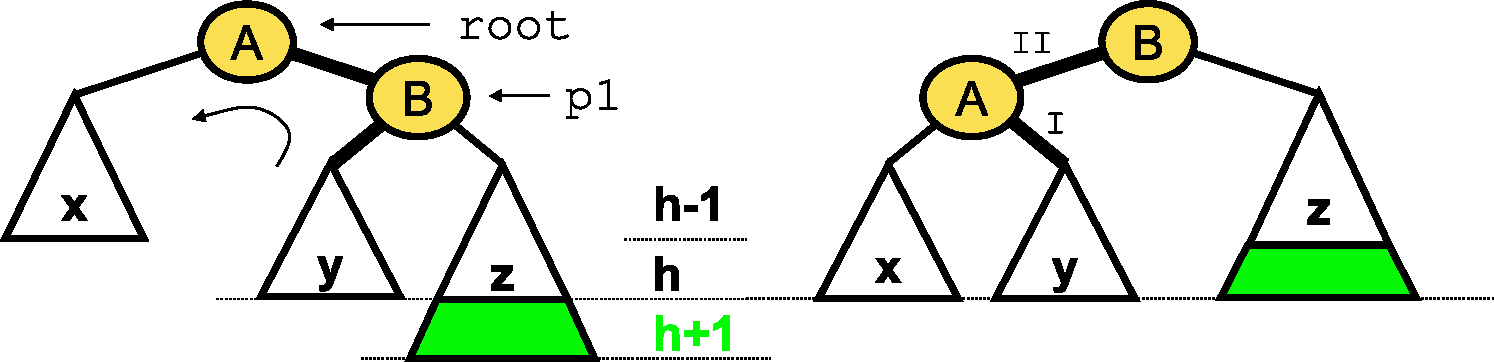
\includegraphics[width=75mm]{03/images/rotace-L}
        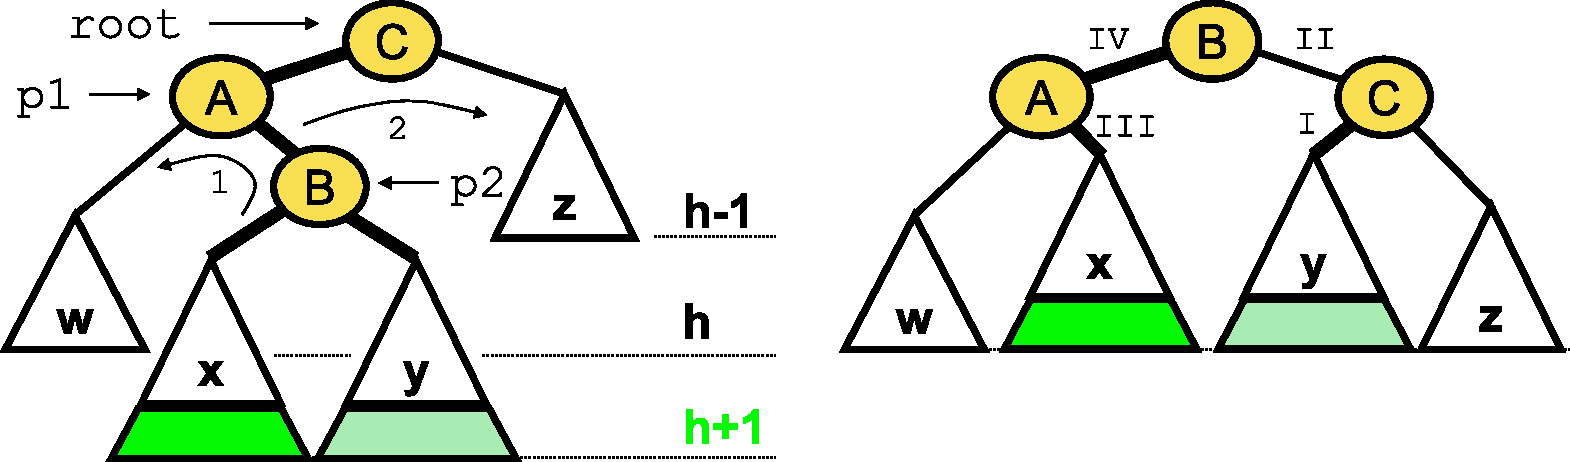
\includegraphics[width=75mm]{03/images/rotace-LR}
    \end{center}
    \caption{Levá a levopravá rotace}
\end{figure}

AVL jsou výškově vyvážené stromy.

\subsection{Splay strom}
Splay strom je \textbf{samovyvažující} binární vyhledávací strom mající tu vlastnost, že \textbf{prvky}, k nimž se \textbf{nedávno přistupovalo}, jsou \textbf{rychle} znovu \textbf{dostupné}. Provádí základní operace jako vkládání, vyhledávání a odstraňování prvků v amortizovaném čase $O(\log n)$ (výška je $n$ ale amortizovaně jsou složitosti logaritmické). Výhodou oproti (např. AVL) je, že nepotřebuje udržovat další informaci (výška nebo barva).

Všechny obvyklé operace na binárních vyhledávacích stromech jsou spojeny s jednou základní, které se říká \textit{splay}. Splay uzlu přeuspořádá strom tak, že se daný uzel dostane do kořene. Způsob, jak toho docílit, je provést standardní vyhledávání daného uzlu v binárním stromu a následně provést speciální rotace stromu takové, aby se uzel dostal do kořene. Každý přístup nebo vložení přendá prvek do rootu. \textit{Zig-Zag} a \textit{Zig-Zig} rotace.

\subsection{R-B (Red-Black) strom}
Červeno-černý strom je binární vyhledávací strom. Je vyvážený, jeho hloubka je maximálně dvojnásobek hloubky vyváženého stromu. Jedná se o datovou strukturu často používanou pro implementaci asociativního pole.

Červeno-černý strom musí splňovat následující pravidla:
\begin{itemize}[itemsep=0px]
\item Každý vrchol je buď červený, nebo černý.
\item Kořen je černý.
\item Listy (nil) jsou pokládány za černé vrcholy.
\item Každý červený vrchol má dva černé syny.
\item Každá cesta z jednoho vrcholu do jeho podřízených listů obsahuje stejný počet černých vrcholů.
\end{itemize}

\paragraph{Černá výška} vrcholu \texttt{x} je počet černých vrcholů na cestě z \texttt{x} k listu (nepočítá se vrchol samotný).

\begin{figure}[h]
    \begin{center}
        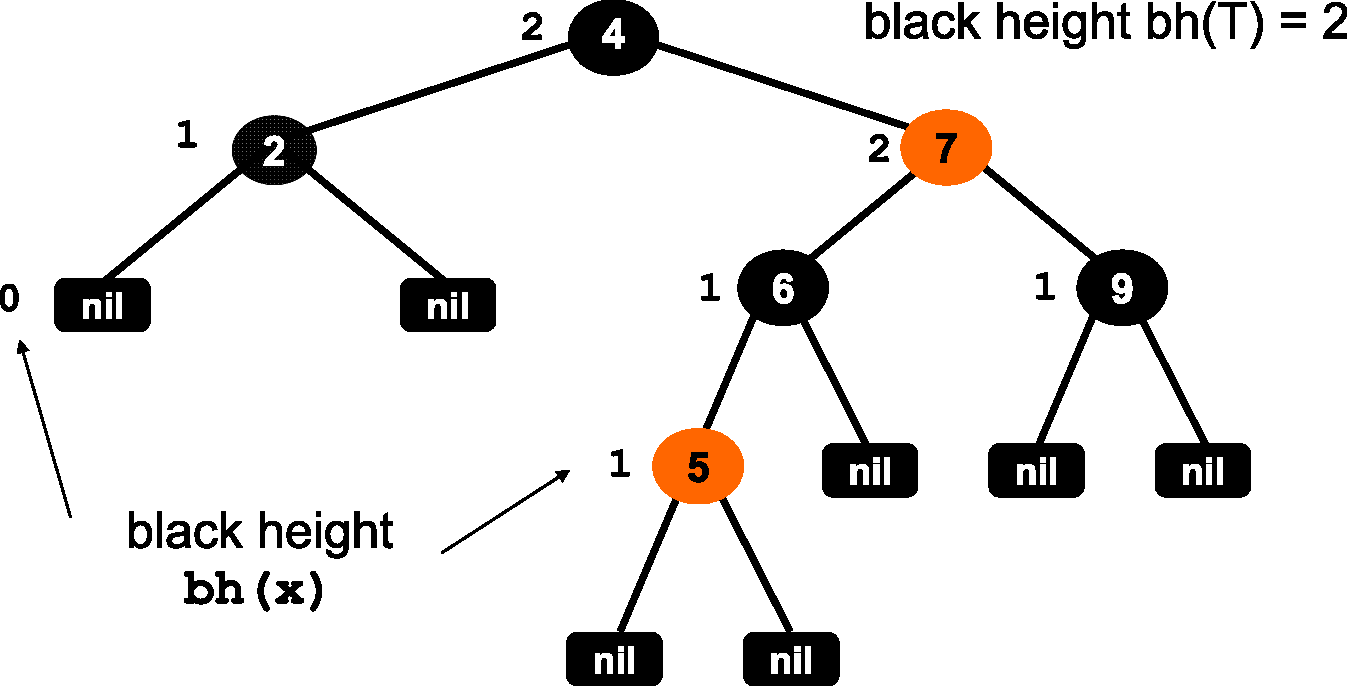
\includegraphics[width=100mm]{03/images/red-black}
    \end{center}
\end{figure}

\paragraph{Vkládání $O(\log(n))$ (max 2 rotace)} Nový node \texttt{x} je červený. Vloží se normálně jako v klasickém BST. Pokud je rodič černý, vše je ok. Pokud je rodič červený:

\begin{itemize}
\item jestli je strýc (nodu \texttt{x}) červený - přebarvení
\item jinak jestli je \texttt{x} pravý potomek  - dvojitá rotace (první rotací se z toho stane 3. případ) + přebarvení
\item jinak jednoduchá rotace + přebarvení
\end{itemize}

\paragraph{Mazání $O(\log(n))$ (max 3 rotace)} Najde se vrchol ke smazání a klasicky se smaže (může mít max 1 potomka, jinak ho zaměníme s s nejblížším předchůdcem a pak ho mažem z nové pozice). Pokud je mazaný prvek červený, můžeme ho v klidu smazat - strom stále zůstane R-B.

Nyní předpokládejte, že mazaný prvek je černý a \texttt{X} je označení potomka mazaného (černého) prvku. Pokud je \texttt{X} červený, stačí ho obarvit na černo a tím je konec. Pokud je černý, tak nastávají 4 případy:

\begin{itemize}
\item pokud je sourozenec červený - levá rotace pravého podstromu, přebarvi sourozence a pokračuj do dalšího případu
\item černý sourozenec s 2 černými potomky - obarvi sourozence a jdi (\texttt{X}) nahoru (double černá barva obarví rodiče)
\item černý sourozenec s min 1 červeným potomkem
\begin{itemize}
\item levý potomek je červený - pravá rotace sourozence (transformuje na následující případ)
\item pravý potomek je červený - levá rotace pravého podstromu
\end{itemize}
\end{itemize}


\subsection{B strom}
B-strom je \textbf{zobecněním BST} v tom smyslu, že umožňuje více než 2 potomky. Je specifický tím, že má řád $n$ a limity na maximální ($n$), i minimální ($\left \lceil \frac{n}{2} \right \rceil$) počet potomků vrcholu. B-strom je díky této vlastnosti \textbf{vyvážený}, operace přidání, vyjmutí i vyhledávání tedy probíhají v logaritmickém čase. Tato struktura je často používána v aplikacích, kdy není celá struktura uložena v paměti RAM, ale v nějaké sekundární paměti, jako je pevný disk (například \textbf{databáze}). Protože přístup do tohoto typu paměti je náročný na čas (hlavně vyhledání náhodné položky), snažíme se minimalizovat počet přístupů do této paměti.

B-strom řádu $n$ je takový strom, který splňuje tyto vlastnosti:

\begin{itemize}[itemsep=0px]
\item Všechny listy (tj.uzly které nemají žádné potomky) jsou na stejné úrovni (ve stejné hloubce).
\item Všechny uzly kromě kořene mají maximálně $n$ a minimálně $\left \lceil \frac{n}{2} \right \rceil$ potomků.
\item Kořen má nejvýše n potomků, spodní hranice není omezena.
\end{itemize}

\paragraph{Princip uložení dat}
Data jsou ve stromu uložena jako setříděné hodnoty, které rozdělují strom na jednotlivé podstromy. Například pokud nějaký uzel má tři potomky, musí být v tomto uzlu uloženy dva klíče $k_1$ a $k_2$, které budou uzel rozdělovat. Všechny hodnoty které jsou menší než $k_1$ musí být uloženy v levém podstromu, hodnoty které jsou větší než $k_1$ a menší než $k_2$ musí být uloženy v prostředním podstromu, a konečně všechny hodnoty větší než $k_2$ musí být v pravém podstromu. Na tyto podstromy jsou samozřejmě v uzlu uloženy ukazatele.

List tedy obsahuje $\left \lceil \frac{n}{2} \right \rceil -1$ až $n-1$ klíčů a neobsahuje žádný ukazatel na podstrom. Vnitřní uzel (tj. takový uzel, který není listem ani kořenem) obsahuje stejný počet klíčů $k$, ale tyto klíče rozdělují potomky tohoto uzlu do $k+1$ podstromů.
Kořen má maximálně $n-1$ klíčů a nemusí mít žádné potomky - v tom případě je pak zároveň listem.

Pokud chceme vložit nebo smazat data (klíče) z uzlu, změní se tím počet potomků tohoto uzlu. Aby se dodržel rozsah daný řádem stromu, vnitřní uzly se v případě potřeby rozdělují či slučují.

\paragraph{Vkládání} Multi vs single fáze strategie vkládání

\begin{figure}[h]
    \begin{center}
        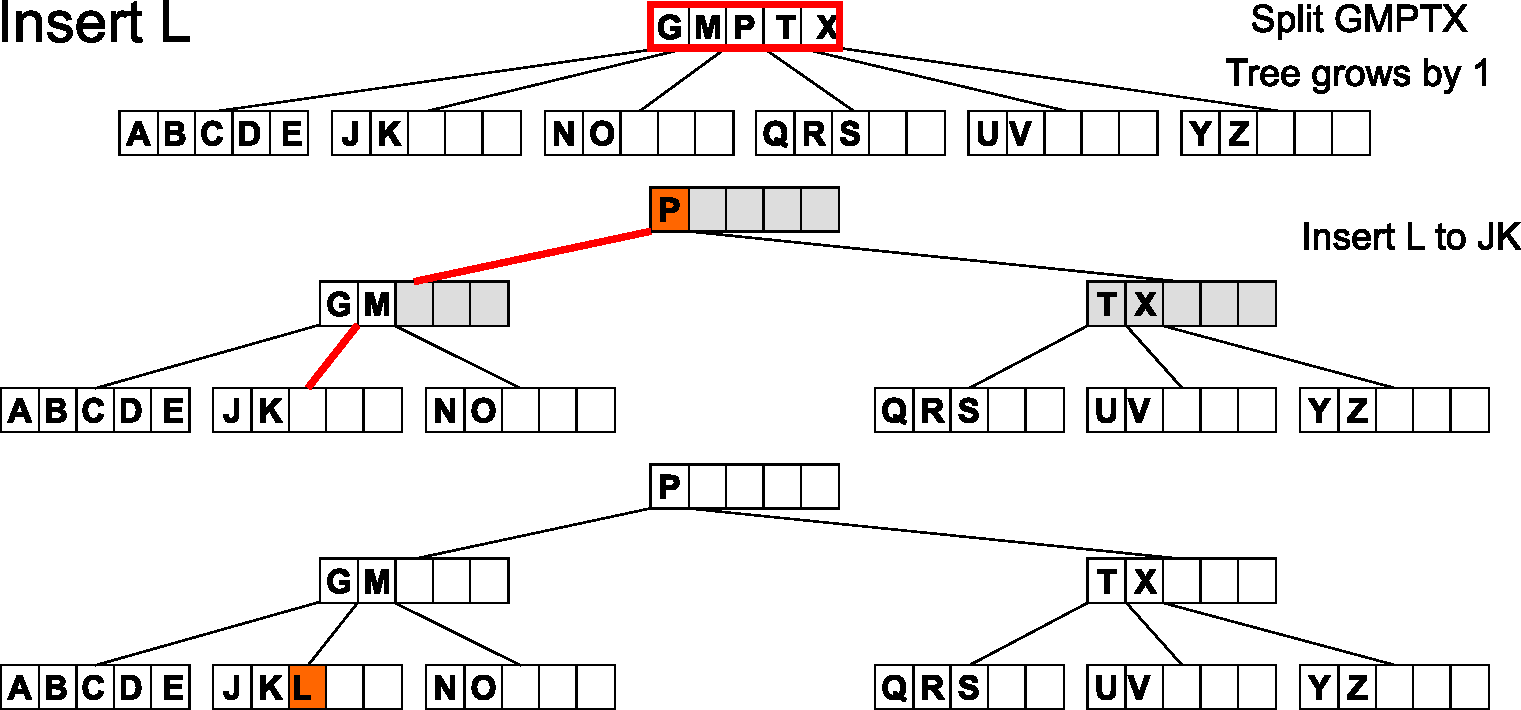
\includegraphics[width=130mm]{03/images/btree-insert}
    \end{center}
    \caption{singlephase strategie vkládání (\uv{avoid the future problems})}
\end{figure}

\paragraph{Mazání} jen multipass strategie!

\begin{figure}[h]
    \begin{center}
        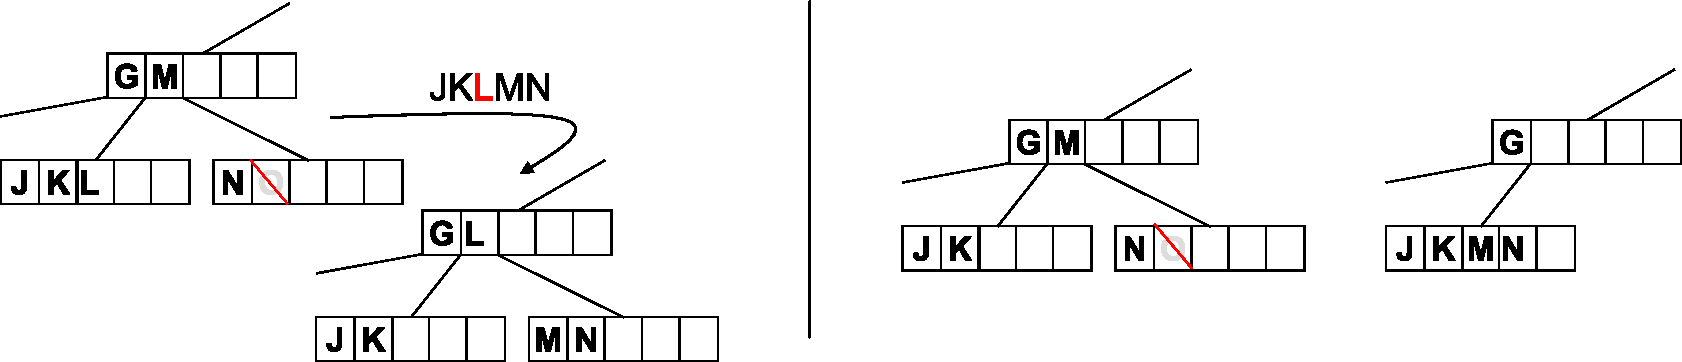
\includegraphics[width=140mm]{03/images/btree-delete}
    \end{center}
\end{figure}

\subsection{2-3-4 strom}
2-3-4 vyhledávací strom je buď prázdný nebo obsahuje 3 typy prvků:

\begin{itemize}
\item \textbf{2}-nody s jedním klíčem, levým odkazem na strom s menšími klíči a pravým odkazem na strom s většími klíči.
\item \textbf{3}-nody s dvěma klíči, levým odkazem na strom s menšími klíči, prostředním odkazem na strom s hodnotami mezi a pravým odkazem na strom s většími klíči.
\item \textbf{4}-nody s třemi klíči a čtyřmi odkazy na stromy s klíči s hodnotami mezi.
\end{itemize}

Všechny odkazy na prázdné stromy (např. listy) mají stejnou vzdálenost od kořene - strom je \textbf{perfektně vyvážený}. Vkládání (s mírným vylepšením) a mazání je stejné jako v B-stromu.

\textbf{2-3-4 strom je strukturou stejný jako B-strom řádu 4.}

\begin{figure}[h]
    \begin{center}
        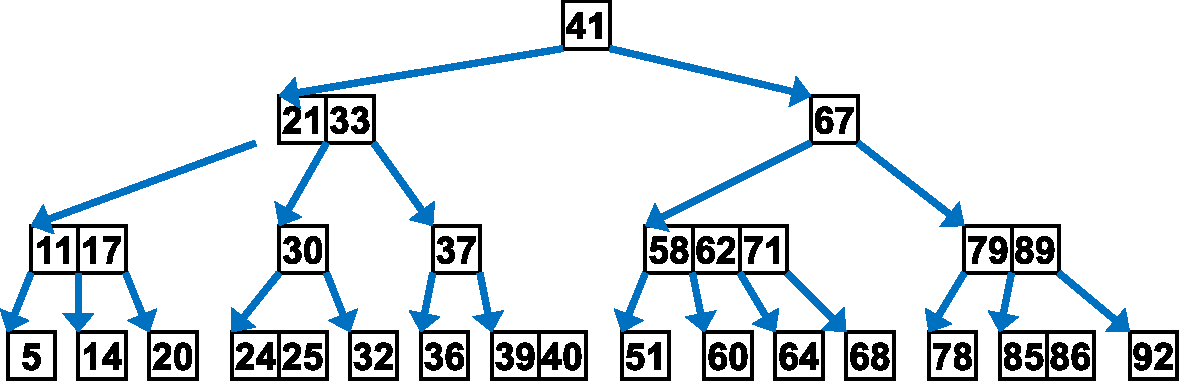
\includegraphics[width=130mm]{03/images/234tree}
    \end{center}
\end{figure}

\subsection{B+ strom}
\textbf{Podobný B-stromu (vždy perfektně vyvážený)} s rozdíly: \textbf{Hodnoty} jsou uloženy \textbf{jen v listech}. Interní prvky obsahují jen vyhledávací klíče a jsou použity jen jako placeholdery k nasměrování hledání.

Listy jsou spolu linkovány ve formě LinkedListu. Hodnoty pak mohou být získány sekvenčně bez přístupu skrze strom.

\begin{figure}[h]
    \begin{center}
        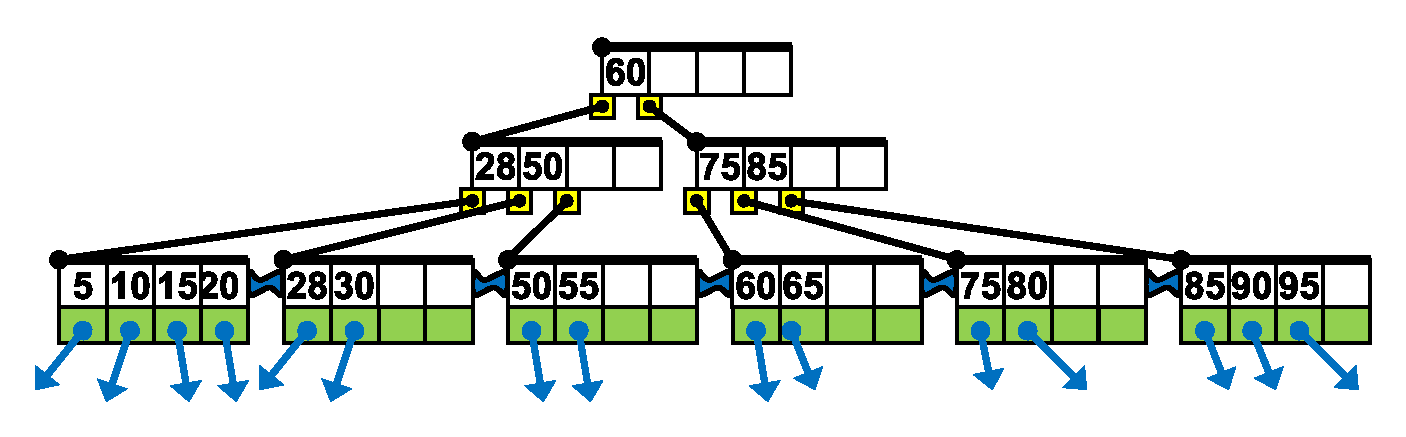
\includegraphics[width=130mm]{03/images/bplustree}
    \end{center}
\end{figure}

Find, Insert, Delete - $\Theta(\log_b n)$ - $b$ je řád stromu, $n$ je počet prvků


\subsection{Vyhledávání ve více dimenzích}

\subsection{K-D strom}
Je BVS reprezentující obdélníkovou plochu v D-dimenzionálním prostoru. Plocha je rozdělena (a rekurzivně dorozdělena) do obdélníkových buněk. Dimenze jsou značeny podle jejich indexu $0,1,\hdots,D-1$.

$R$ je kořen stromu (nebo podstromu). Obdélníková D-dimenzionální buňka $C(R)$ (hyperobdelník) je asociován s $R$. Jsou definovány souřadnice $R[0],R[1], ..$ a hloubka stromu $h$.

\begin{figure}[h]
    \begin{center}
        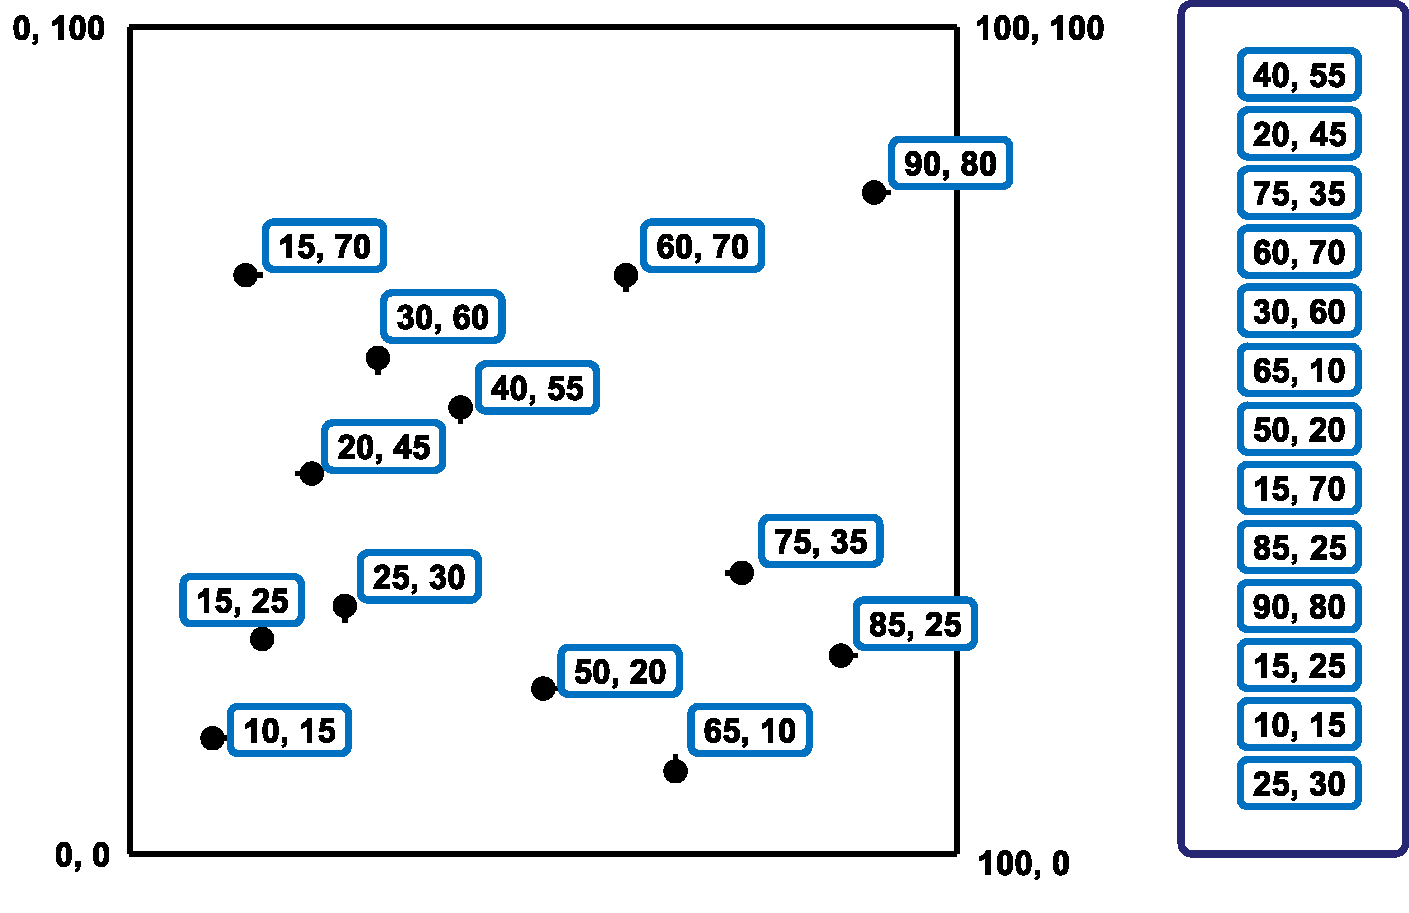
\includegraphics[width=130mm]{03/images/kdtree01}
        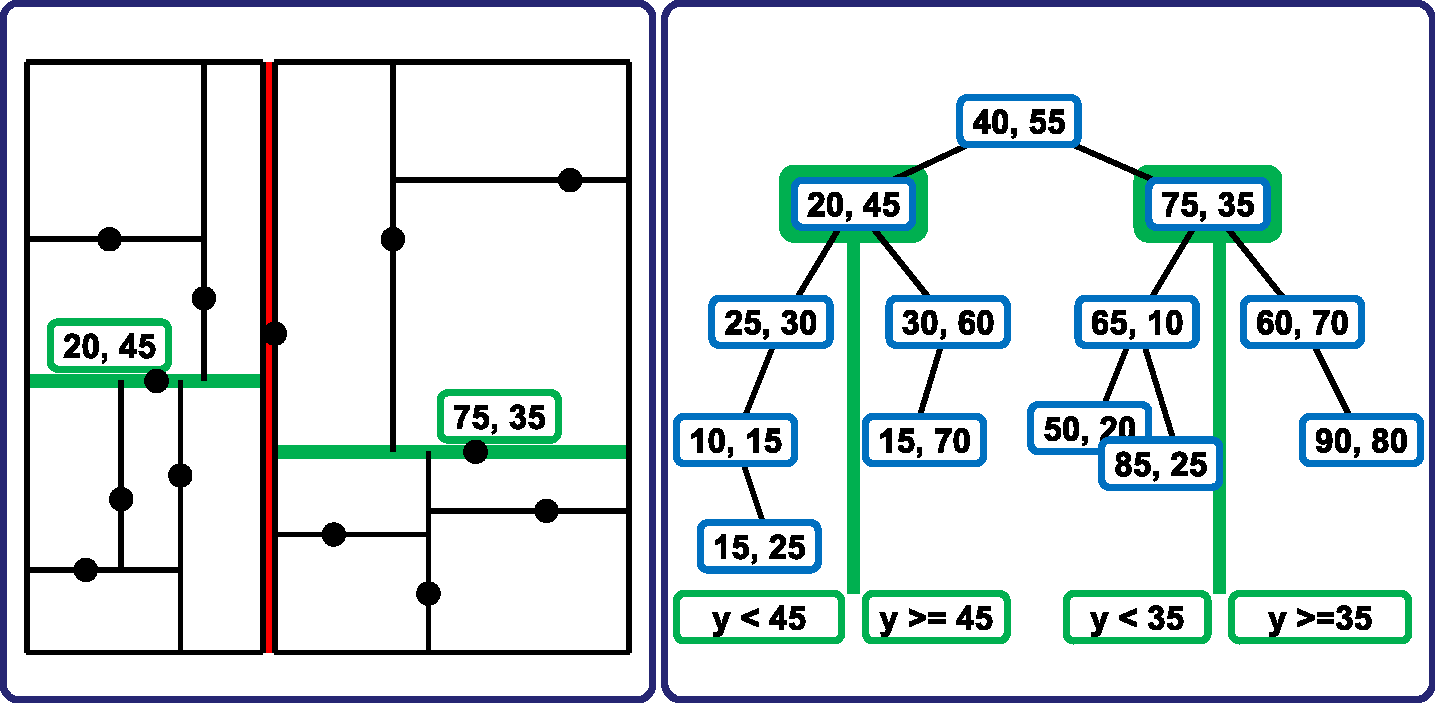
\includegraphics[width=130mm]{03/images/kdtree02}
    \end{center}
\end{figure}

\paragraph{Operace}
\begin{itemize}
\item \textbf{Find(key)} - stejné jako v 1D stromě. Hledá se střídavě podle souřadníc odpovídající hloubce stromu (modulo) a postupně se osekává vyhledávaný prostor.

\item \textbf{Insert(key)} - stejné jako v 1D stromě. Porovnávají se střídavě souřadníce odpovídající hloubce stromu (modulo) a postupně se projde až k listu, kam se nový prvek vloží.

\item \textbf{FindMin(dim)} - minimální prvek pro určitou dimenzi. Tato operace je provedena jako část operace delete. Nejnáročnější operace (protože delete metoda rapidně mění strukturu stromu) - $O(n^{1-1/d})$.

\item \textbf{Delete()} - jen listy mohou být smazány. Mazání prvku uvnitř stromu je zajištěno náhradou hodnot, za hodnoty jiného odpovídajícího prvku hlouběji ve stromu. Pokud pravý podstrom R není prázdný, najdi v něm minimum (podle dimenze hledaného prvku). Pokud je prázdný hledej v levém podstromu (podle dimenze hledaného prvku).
\end{itemize}

\subsection{Skip List}
Je seřazený linkedlist kde každý prvek obsahuje proměnný počet odkazů. $k$-tý link implementuje jednoduchý linkedlist, který přeskakuje prvky s menším počtem linků než $k$.

Je to LinkedList s vyhledávací náročnosti $O(\log(n))$. Problém má navazujícími insert/delete operacemi - ty ničí \uv{správný} tvar listu a tím. Řešením je vytvořit náhodný tvar podobný tomu optimálnímu, malé náhodné deviace v dlouhém běhu využití struktury nám tolik nevadí.

\begin{itemize}
\item \textbf{find} - postupně se prochází top-level listy a postupně se míří níže.
\item \textbf{insert} - opět se postupně prochází níže až se vloží nový prvek a náhodně se vygeneruje $k$ pro nově vzniklý prvek - doplní se linky na ostatní prvky.
\end{itemize}

\begin{figure}[h]
    \begin{center}
        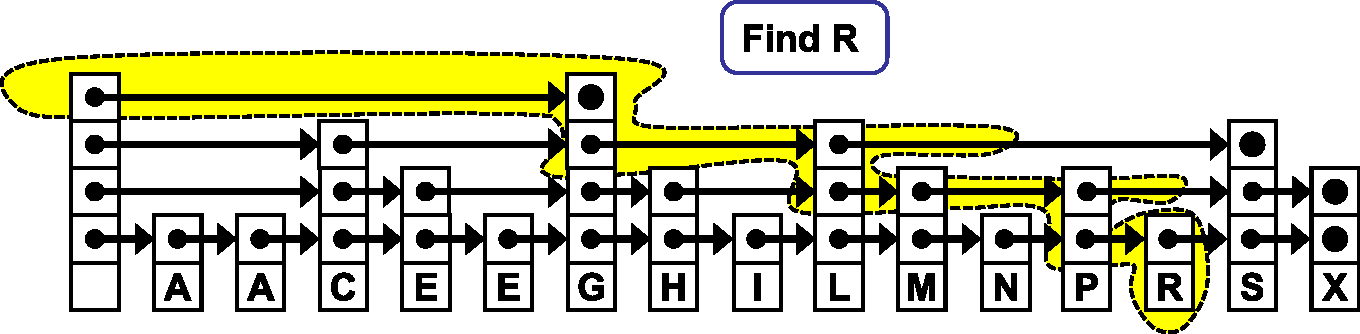
\includegraphics[width=130mm]{03/images/skiplist}
    \end{center}
\end{figure}